\documentclass[11.8pt]{amsart}
\usepackage[margin=3cm]{geometry}                % See geometry.pdf to learn the layout options. There are lots.
\geometry{letterpaper}                   % ... or a4paper or a5paper or ...
%\geometry{landscape}                % Activate for for rotated page geometry
\usepackage[parfill]{parskip}    % Activate to begin paragraphs with an empty line rather than an indent
\usepackage{float}
\usepackage{graphicx}
\usepackage{amssymb}
\usepackage{epstopdf}
\usepackage{siunitx}
\usepackage{subcaption}
\usepackage{setspace}

\setstretch{1.3}

\DeclareGraphicsRule{.tif}{png}{.png}{`convert #1 `dirname #1`/`basename #1 .tif`.png}
\graphicspath{{img/}}

\title{Lab 9: Spectroscopy}
\author{Caspar \textsc{Lant}} % Author name

\date{\today} % Date for the report

\begin{document}

\bigskip

\maketitle % Insert the title, author and date
\begin{center}

Intermediate Experimental Physics I\\
\vspace{1.5cm}

\begin{tabular}{l r}

Section: & 002\\
\\
Date Performed: & December 2, 2015 \\ % Date the experiment was performed
Date Due: & December 9, 2015\\
\\
Partner: & Sam P. Meier \\ % Partner names
Professor: & Prof. Andrew Kent\\
Instructor: & David Mykytyn % Instructor/supervisor
\end{tabular}
\end{center}
\vspace{50mm}
\pagebreak

\paragraph{\textbf{The Objective} of this week's experiment was to put our vast theoretical knowledge of lenses to application. It is always a remarkable think to see what was once pure abstraction validated though rigorous scientific experimentation. }

\section{Theoretical Background/ Abstract}
\paragraph{Last weeek we discovered that light propegates as a wave. As we know, one of the ways in which we define waves is by their frequency of wavelength. In the case of light waves, it is frequency that determines the color of an incident light wave, and whether or not it is visible to us humans. It turns out that gases---as well a other incandescent solids---when excited with en electric current, tend to emit light of particular frequency, depending on the nature of the gas. This is given by the following equation, where $E$ is the energy difference between energy levels in the atoms or molecules of the gas:}
\begin{equation}
E = hv
\end{equation}
\paragraph{The greek letter $\nu$ is commonly used to denote the frequency of an electromagnetic wave, as it does in this case. Don't ask me why this is--I find it very confusing. The letter $h$ in this equation denotes Plank's constant, which has an approximate value of $6.6 \times 10^{34} \ \text{J $\cdot$ s} $. Anyways, each energized gas that we decide to put in front of our spectrometer will emit a unique array of spectra at particular frequencies, which will allow us to identify the gas. But first, how does a spectrometer work!? We know that light of different frequencies will refract at different angles when passing through a material boundary. We have ignored this fact up until now, but it is nethertheless true. What allowed us to ignore it in previous lab experiments and calculations was that we were dealing with coherent planes of light, of homogenous wavelength and frequency. At the very least, the light that we observed fell within the frequency range of light visible by humans. The device that we use in this experiment, called a "light sensor," is sensitive to a range of frequencies greater than that of us piddly humans. We will send our light through two lenses in order to further separate the light waves of disparate frequency, but not before it is diffracted by our \textit{diffraction grating}, whos slit width we will calculate. Recall from our experiments on diffraction interference that this width, for a grating with multiple apertures (slits) is given by the following equation:}
\begin{equation}[H]
d\sin\theta = m\lambda (m = 0, \pm1, \pm2, \ ...)
\end{equation}
\paragraph{The width of these slits, as well as the distance between slits on a quality diffraction grating is often on the order of hunderds or thousands of nanometers, or one-ten-millionth of a meter. The number of slit per unit length of this grating largely determines its resolving power, which is a quantitative measure of how far apart two waves have to be, in wavelength, to be distinguished on the screen of the spectometer:}
\begin{equation}
R = \dfrac{\lambda}{\Delta\lambda} = mN
\end{equation}
\newpage
\section{Experimental Procedure}
\begin{enumerate}
\item Begin by setting up the experiment as shown in the above diagram. You should make sure that all lenses and diffraction gradients are perpendicular the the axis of incoming light rays.
\item Make doubly sure that the diffraction grating mounted to the protractor is oriented at zero degrees.
\item Connect the rotary motion sensor and the light sensor to DataStudio, and set up the appropriate graphs and tables.
\item Place the sodium lamp at the helm of the experimental boondoggle (apparatus)
\item It may help to place a slitted shade in the path of the sodium lamp to mitigate "leakage" of ambient light. This is a good place to tell you that you should be conducting your experiment in a darkened room.
\item Turn on the sodium lamp and focus the central maxima by changing the position of the image lens.
\item Rotate the protractor such that the (faint) second-order line appears on the screen.
\item Begin your experiment in DataStudio and rotate the the screen in the direction of 0$^{/circ}$, all the way around to the furthest second-order line.
\item Your graph in DataStudio should have picked up on all the spectra apparent on the screen, as well as perhaps some invisible lines, as discussed in the previous section.
\item Repeat the experiment with the sodium lamp a few more times, and then with each new bulb.
\item Use the graphs of each gas, as well as the ratio of rotation between the spool and platter, to calculate the angle of each spectral artifact.
\item From these angles, calculate the wavelength of each artifact using the double-slit formula (2)
\item Use the collection of wavelengths for each gas to determine the composition of each gas.
\end{enumerate}
\vfill
\section{Questions}

\begin{enumerate}
\item {\textit{What are appropriate units for $d$ and $\lambda$? For $\theta$?}

\begin{quote}
$d$ and $\lambda$ are both appropriately measured in units of length Nanometers seem to be on the right order of magnitude. Angles $\theta$ are, of course, measured in degrees or radians, but because we make the paraxial assumption $\theta\approx\sin\theta\approx\tan\theta$, it is also fine to treat these angles as dimensionless.\end{quote}}
\item{\textit{Calculate the wavelengths of lines X. Why do you not see them on the screen?}
\begin{quote}
The wavelengths that correspond to each bright line X fall outsude of the frequency range of light visible by humans, but not--of course--by the spectrometer.
\end{quote}}
\end{enumerate}
\vfill\newpage

\newgeometry{left=.75cm,right=0.25cm,  bottom=1.25cm}
% \section{Graphs}
\begin{figure}[H]
    \begin{minipage}{.5\textwidth}
        \caption{Sodium}
        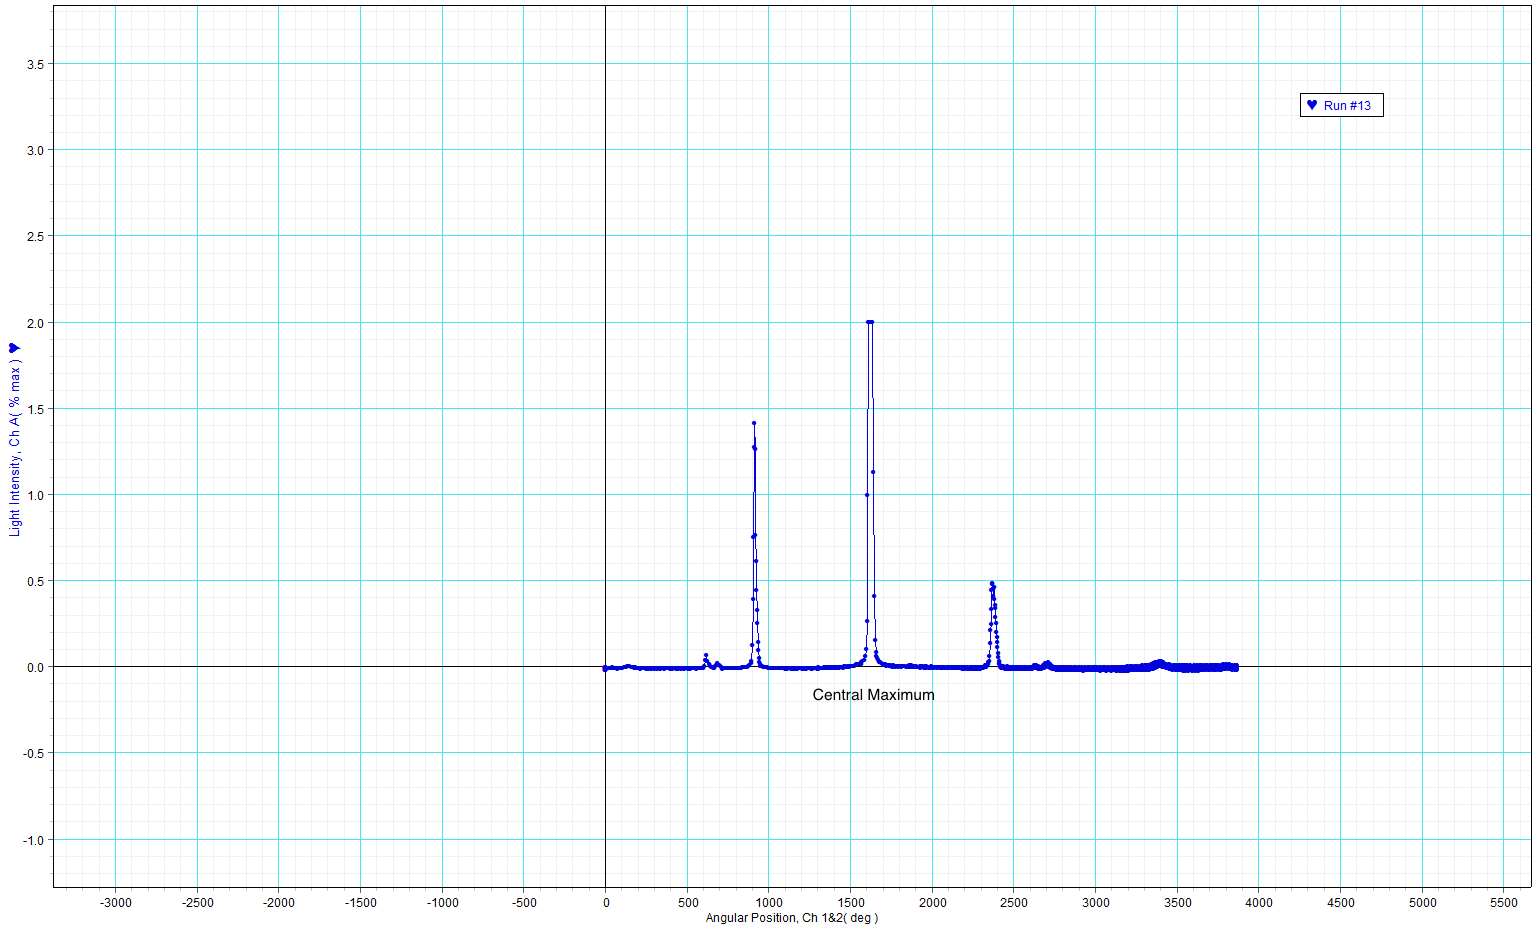
\includegraphics[height=2.3in]{sod.png}
    \end{minipage}%
    \begin{minipage}{.5\textwidth}
        \caption{Helium}
        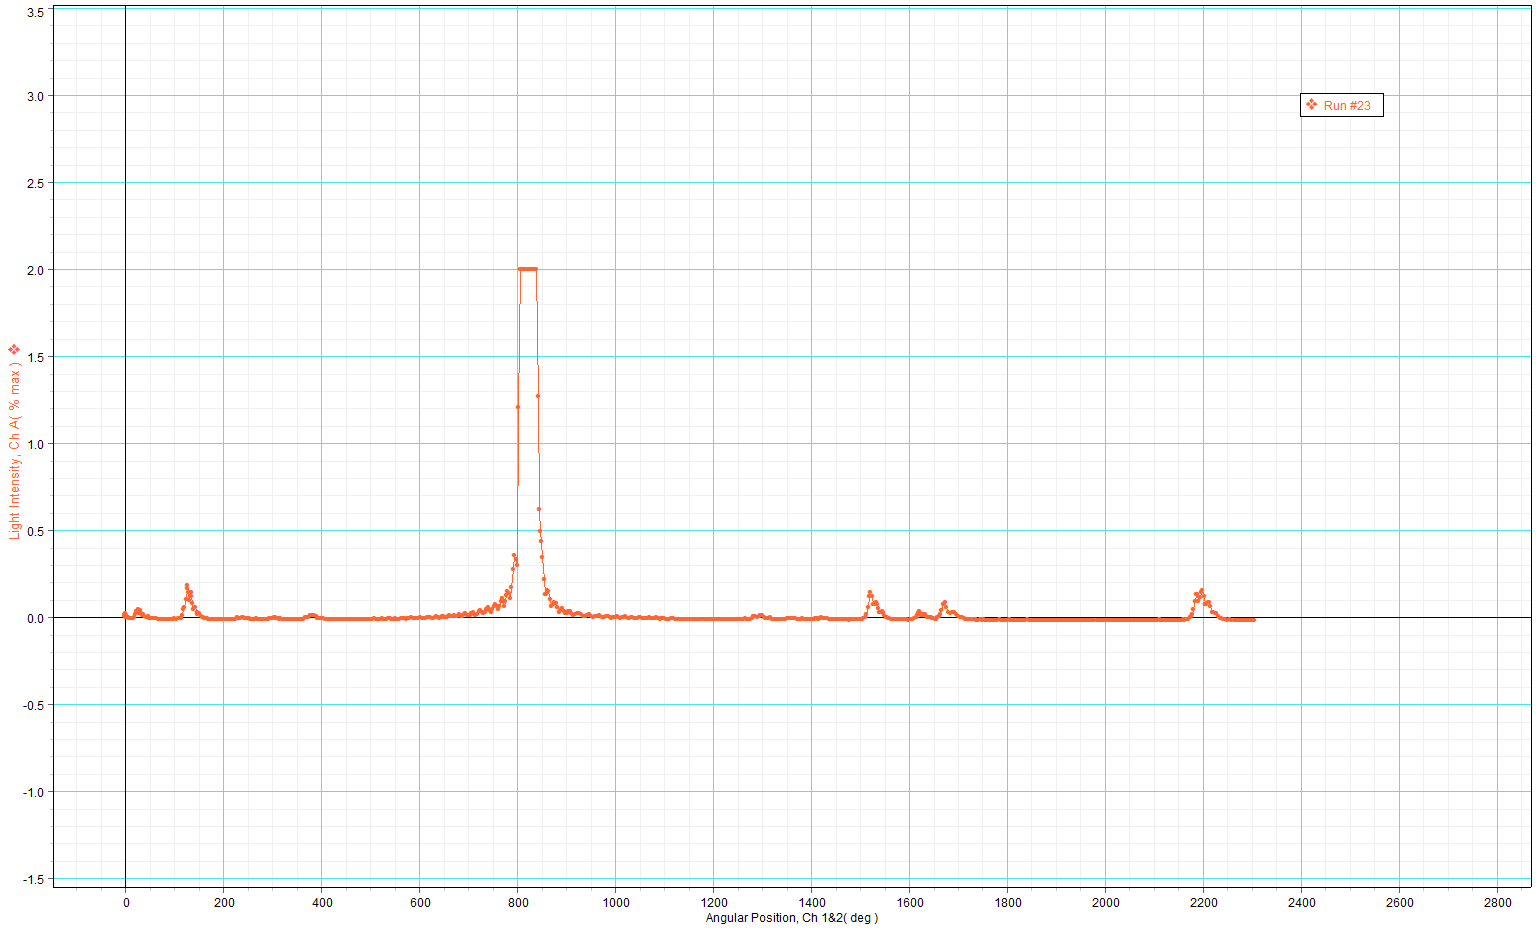
\includegraphics[height=2.3in]{he.png}
        %\caption*{maybe put the frequecies here?}
    \end{minipage}
\end{figure}
\vfill
\begin{figure}[H]
    \begin{minipage}{.5\textwidth}
        \caption{Hydrogen}
        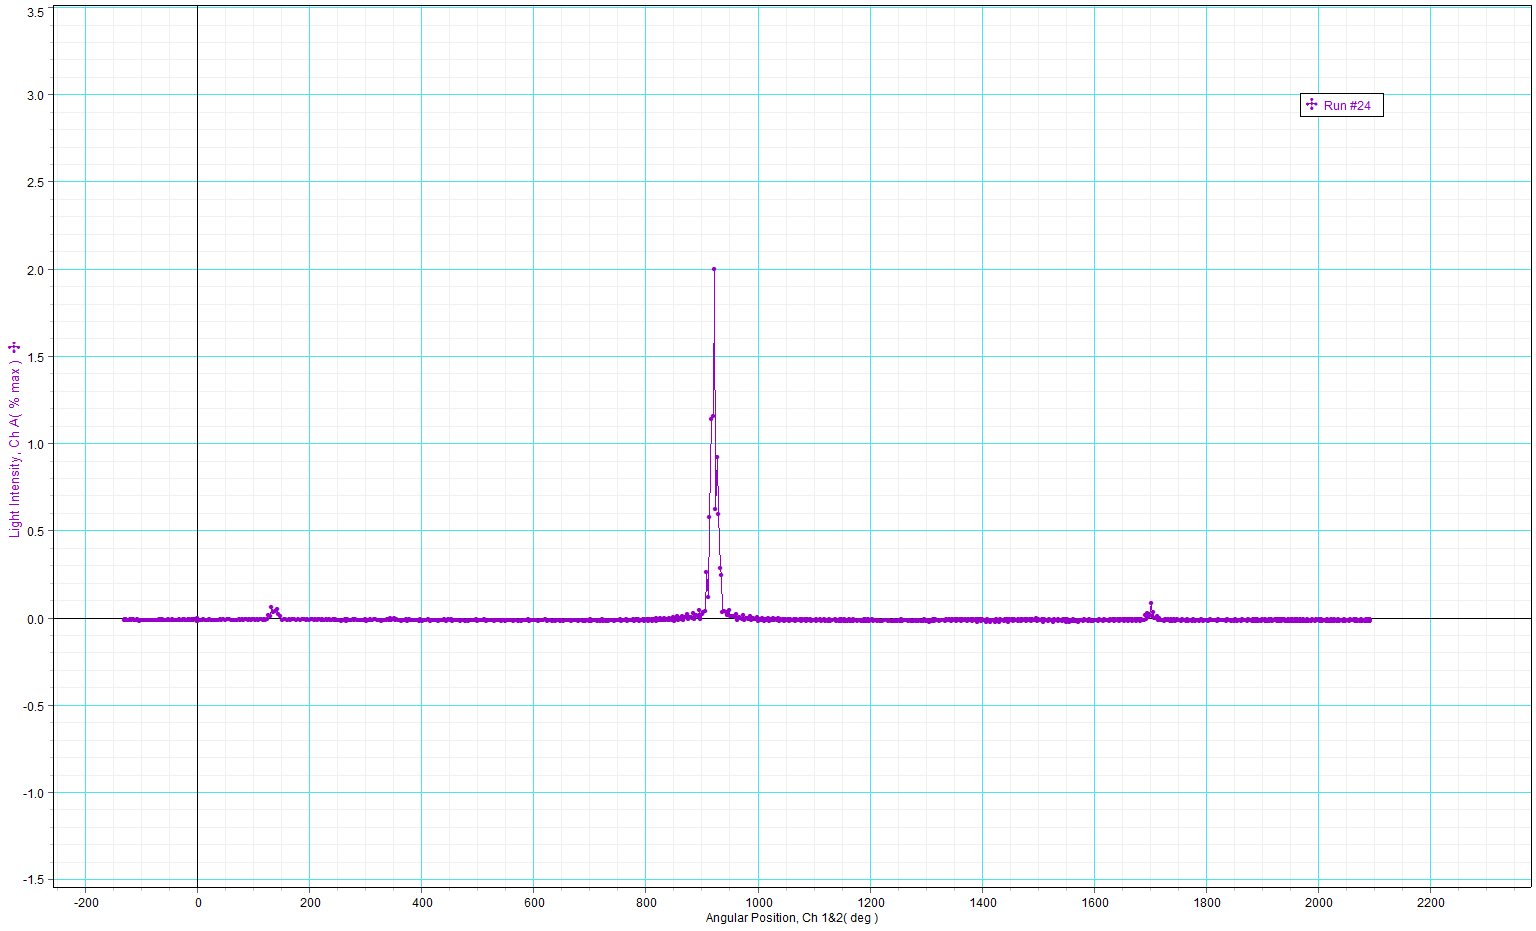
\includegraphics[height=2.3in]{hy.png}
    \end{minipage}%
    \begin{minipage}{.5\textwidth}
        \caption{Water}
        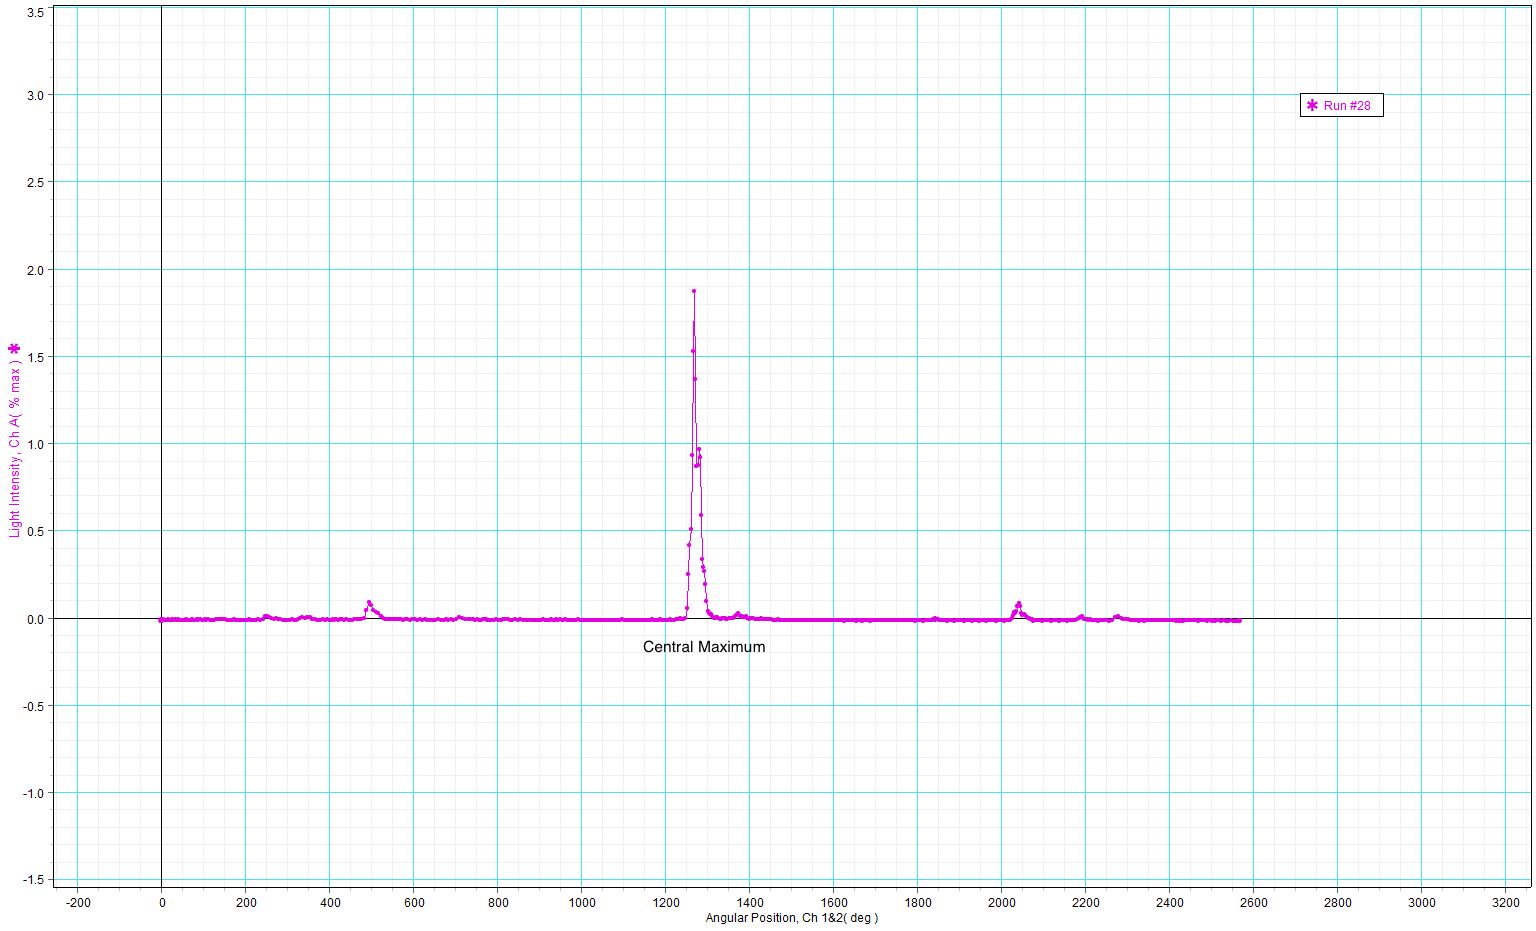
\includegraphics[height=2.3in]{water.png}
    \end{minipage}%
\end{figure}
\vfill
\begin{figure}[H]
    \begin{minipage}{.5\textwidth}
        \caption{Mystery}
        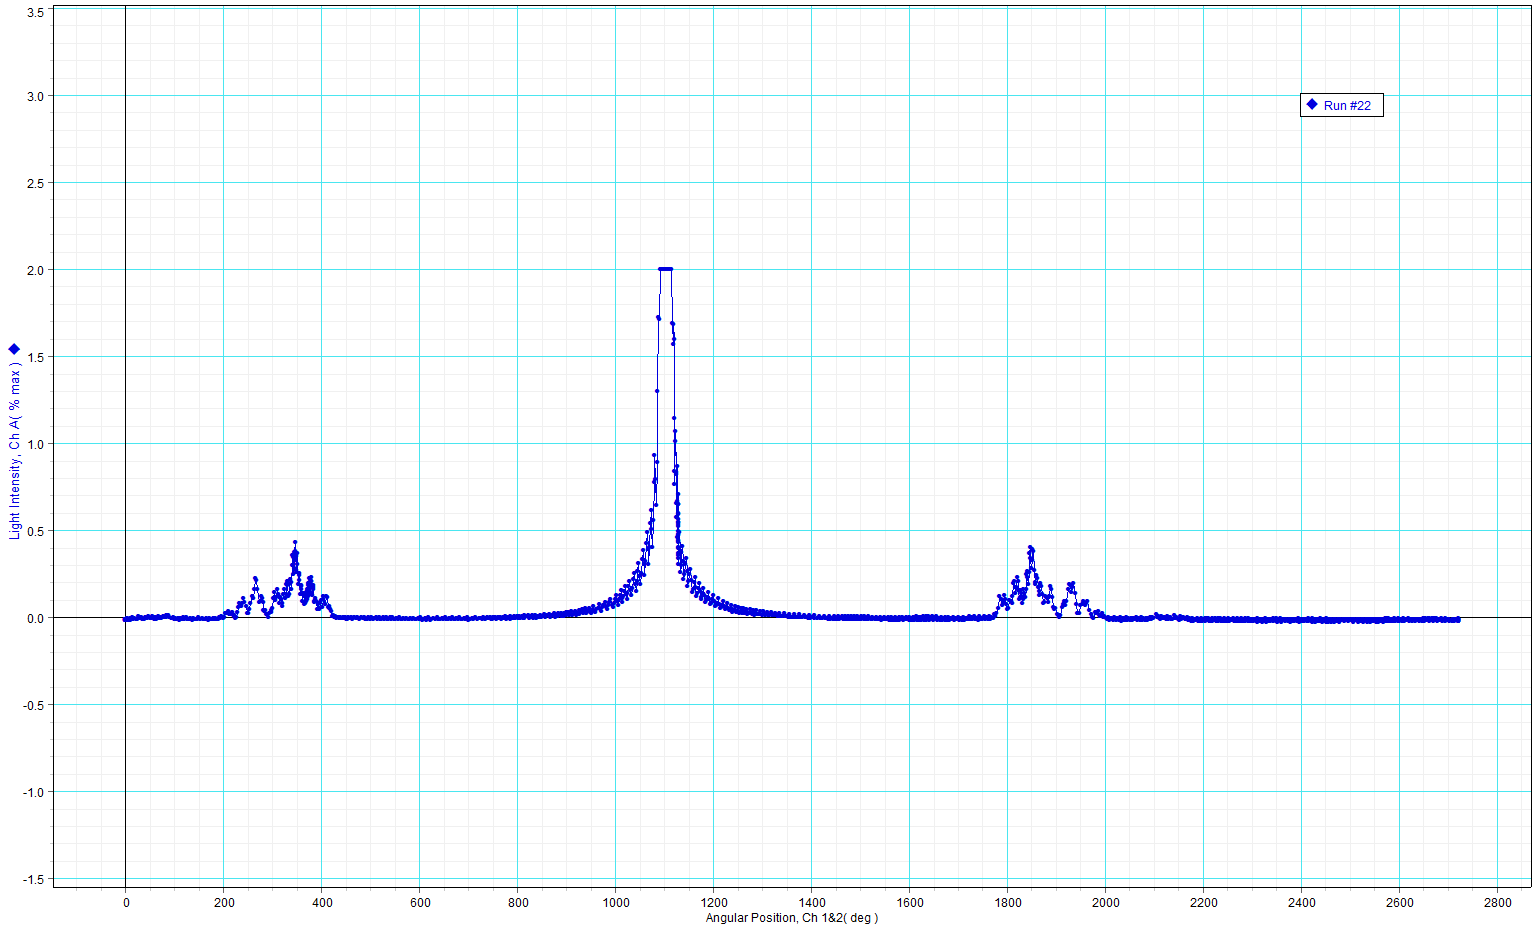
\includegraphics[height=2.3in]{myst.png}
    \end{minipage}%
    \begin{minipage}{.5\textwidth}
        \caption{Neon}
        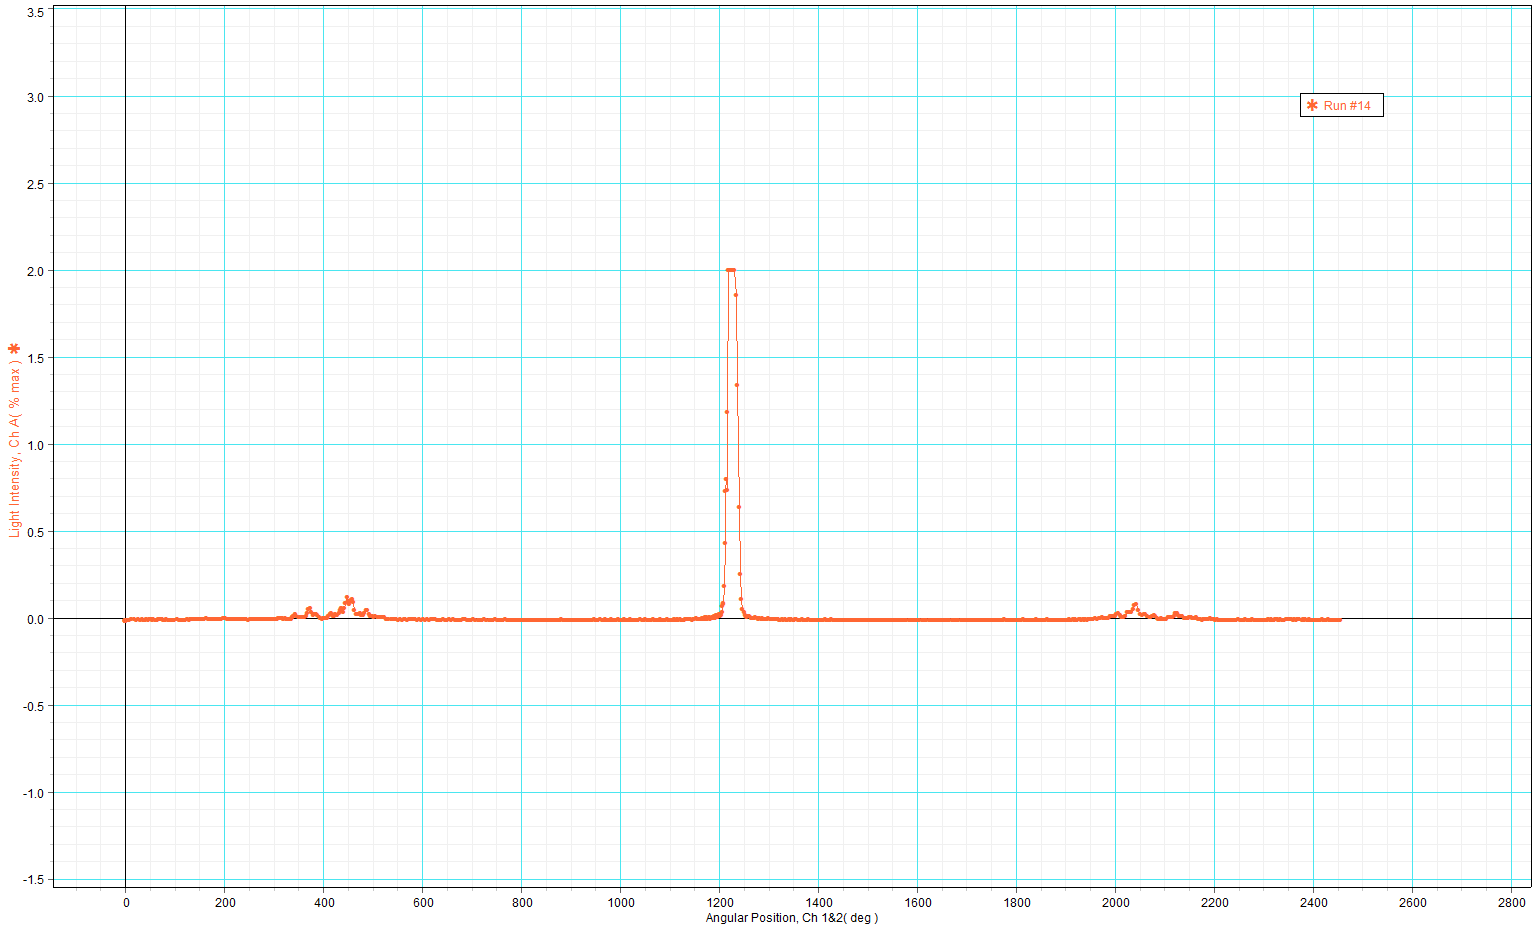
\includegraphics[height=2.3in]{neon.png}
    \end{minipage}%
\end{figure}
\vfill
\restoregeometry
\newpage

\section{Tables}
\begin{table}[H]
\centering
\setstretch{1}
\caption{Angles of Spectra From Graph}
\label{my-label}
\begin{tabular}{r|c|c|c|c|c|c|c|c|c|c}
Gas      & Central Maximum & 0     & 1'    & 2'   & 3' & 4'  & 5'   & 6'   & 7'  & 8'   \\\hline
Sodium   & 1620            &       & -1020 & -720 & 0  & 755 & 1080 & 1780 &     &      \\
Helium   & 825             &       & -700  & -450 & 0  & 475 & 700  & 800  & 850 & 1375 \\
Hydrogen & 920             &       &       & -780 & 0  & 780 &      &      &     &      \\
Water    & 1265            & -1015 & -915  & -765 & 0  & 835 & 935  & 1010 &     &      \\
Mystery  & 1100            & -940  & -750  & -700 & 0  & 680 & 750  & 825  & 855 &      \\
Neon     & 1225            &       & -850  & -775 & 0  & 815 & 900  &      &     &
\end{tabular}
\end{table}

\begin{table}[H]
\centering
\setstretch{1}
\caption{Angles of Spectra (Corrected)}
\label{my-label}
\begin{tabular}{r|c|c|c|c|c|c|c|c|c|c}
Gas      & Central Maximum & 0   & 1'  & 2'   & 3' & 4'  & 5' & 6' & 7' & 8' \\\hline
Sodium   & 1620$^{\circ}$            &     & -26$^{\circ}$ & -18$^{\circ}$  & 0$^{\circ}$  & 19$^{\circ}$  & 27$^{\circ}$ & 45$^{\circ}$ &    &    \\
Helium   & 825$^{\circ}$            &     & -18$^{\circ}$ & -11$^{\circ}$  & 0$^{\circ}$  & 12$^{\circ}$  & 18$^{\circ}$ & 20$^{\circ}$ & 21$^{\circ}$ & 34$^{\circ}$ \\
Hydrogen & 920$^{\circ}$            &     &     & -780$^{\circ}$ & 0$^{\circ}$  & 780$^{\circ}$ &    &    &    &    \\
Water    & 1265$^{\circ}$            & -25$^{\circ}$ & -23$^{\circ}$ & -19$^{\circ}$  & 0$^{\circ}$  & 21$^{\circ}$  & 23$^{\circ}$ & 25$^{\circ}$ &    &    \\
Mystery  & 1100$^{\circ}$            & -24$^{\circ}$ & -19$^{\circ}$ & -18$^{\circ}$  & 0$^{\circ}$  & 17$^{\circ}$  & 19$^{\circ}$ & 21$^{\circ}$ & 21$^{\circ}$ &    \\
Neon     & 1225$^{\circ}$            &     & -21$^{\circ}$ & -19$^{\circ}$  & 0$^{\circ}$  & 20$^{\circ}$  & 23$^{\circ}$ &   &    &
\end{tabular}
\end{table}

\begin{table}[H]
\centering
\setstretch{1}
\caption{Experimental Values of Wavelength}
\label{my-label}
\begin{tabular}{r|c|c|c|c}
Gas      & $\frac{1}{2}(\theta_\text{left}-\theta_\text{right})_1$ & $\frac{1}{2}(\theta_\text{left}-\theta_\text{right})_2$ & $\langle d \rangle_\text{slits}$ (nm)  & $\lambda_\text{gas}$ (nm) \\\hline
Sodium   & 18.4$^{\circ}$            & 26.3$^{\circ}$            & 1391.3 & 1021.1   \\
Helium   & 11.6$^{\circ}$            & 17.5$^{\circ}$            & 1391.3 & 1260.6   \\
Hydrogen & 780.0$^{\circ}$            & 0.0$^{\circ}$            & 1391.3 & 1363.8    \\
Water    & 20.0$^{\circ}$            & 23.1$^{\circ}$            & 1391.3 & 1036.7    \\
Mystery  & 17.3$^{\circ}$            & 18.8$^{\circ}$            & 1391.3 & 80.0      \\
Neon     & 19.9$^{\circ}$            & 21.9$^{\circ}$            & 1391.3 & 1234.0
\end{tabular}
\end{table}
\setstretch{1}
\paragraph{As you can see, there's some funky stuff going on here, especially in the case of the "mystery" gas, which turns out to be Hydrogen}

\setstretch{1.1}
\section{Error Analysis}
\paragraph{Calculating the error of my data in this lab is difficult, because I have no expected values for spectra to compare them to. That being said, here is the equation that dictates my uncertainty for wavelength and slit width:}
\begin{equation*}
    \delta \lambda = |\lambda|\sqrt{\left(\frac{\delta d}{d}\right)^2+\left(\frac{\delta \theta}{\theta}\right)^2}
    \ \ \ \leftarrow
    \delta d = |d||\lambda_\text{sodium}|\left( \frac{\delta \text{Rotation Ratio}} {\text{Rotation Ratio}} \right)^2
\end{equation*}
\paragraph{The main source of error in this experiment undoubtably stemmed from the difficulties I had with my rotary motion sensor. You'll see in a few of the graphs that the angle swept is far larger than is typical, even though I moved the protractor plate by a roughly equal distance in each iteration of the experiment. This is compelling evidence of spool slippage! If this were the case, I would have no reliable means of calculating the wavelength of the bright line spectra.  }

\end{document}
